% Suppress some compilation warnings
\RequirePackage[save,showerrors]{silence}
\WarningFilter{biblatex}
  {The starred command '\DeclareDelimAlias*' is} % APA package is using this deprecated starred version
\WarningFilter{transparent}
  {Loading aborted} % Used by the svg package

\documentclass[usenames,dvipsnames,10pt]{beamer}

% languages typesetting rules
\usepackage[main=french,english]{babel}

% links configuration
\usepackage{hyperref} % commands such as \href, \url, etc.
\hypersetup{
    colorlinks=true,
    linkcolor=,
    urlcolor=NavyBlue,
    citecolor=Green
}

% bibliography configuration
\usepackage[style=lncs,backend=biber,backref=true]{biblatex}

\usepackage{csquotes} % biblatex extensions for non-english languages
\usepackage{caption} % more control over captions
\usepackage{subcaption} % for subfigures
\usepackage{ccicons} % icons for Creative-Commons licenses
\usepackage{hologo} % tex and co. logos
\usepackage{siunitx} % for displaying large numbers
\usepackage[inkscapepath=./build/svg-inkscape/]{svg}

\graphicspath{{images/} {../images}}

% Beamer theme configuration
\usetheme{metropolis}
\metroset{sectionpage=progressbar, progressbar=frametitle}
\setbeamertemplate{caption}[numbered] % Show figure number when using `\caption` instead of `\caption*`
\setbeamertemplate{footline}[frame number] % Show the current frame number instead of page number in the bottom line of each slide
% \setbeameroption{show only notes}
\setbeameroption{show notes on second screen}

% Bibliography configuration
\bibliography{../references.bib}

% Meta information about this presentation
\title{L'identification des projets de logiciel libre accessibles aux nouveaux contributeurs}
\titlegraphic{
\includegraphics[width=0.25\textwidth]{EIAH_2023}}
\institute[]{\href{https://creativecommons.org/licenses/by-sa/4.0/}{\ccbysa}}
\author{%
    Paul Hervot\inst{1}%
    \and%
    Benoît Crespin\inst{2}%
}
\institute{
    \textsuperscript{1} Laboratoire de Recherche de L’EPITA (LRE), 14-16 rue Voltaire, \\94270 Le Kremlin-Bicêtre, France
    \and
    \textsuperscript{2} Université de Limoges, XLIM/ASALI, UMR CNRS 7252, France
}
\date{15 juin 2023}

\newcommand{\mycite}[1]{%
    \citeauthor{#1} \citeyear{#1} \cite{#1}%
}

\begin{document}

\frame{\titlepage{}}

\section{Contexte}

\begin{frame}{Mémoire de Master}
    Formation d'ingénieur, enseignant à EPITA.

    Mémoire supervisé par Benoît Crespin.
    
    % Je ne viens pas, à la base, du monde de la recherche, j'ai une formation
    % d'ingénieur et j'enseigne l'informatique depuis six ans. Cet article est
    % en fait le fruit d'un travail de mémoire de M2 que j'ai fait l'année
    % dernière en formation continue et supervisé par mon co-auteur, qui n'a pas
    % pu venir aujourd'hui mais que je remercie beaucoup pour son aide, en
    % particulier quand il a été question de soumettre à cette conférence.
    \note[item]{Profil ingénieur / prof, pas trop recherche}
    \note[item]{Expérience lors d'un travail de mémoire de Master}
\end{frame}

\begin{frame}[fragile]{Contributions au logiciel libre}
    Nombreuses barrières d'accès, souvent discriminantes :
    \mycite{barriers-2018}, \mycite{newcomers-accessibility-2016},
    \mycite{newcomers-onboarding-2018}.

    \bigskip\bigskip

    Souvent liées aux propriétés des projets $\implies$ peut-on identifier
    lesquels sont accessibles ?

    % Ce travail s'inscrit dans la recherche autour des barrières d'accès que
    % les nouveaux contributeurs rencontrent en essayent de contribuer aux
    % projets de logiciel libre. Ce type de contribution est parfois utilisé en
    % cours dans le cadre de la pédagogie de projet mais c'est encore assez
    % rare, en partie à cause de ces barrières justement.

    % Ce sont des barrières qui sont même assez souvent discriminantes, en
    % particulier sur le genre.

    % Notre question est donc de savoir s'il existe des indicateurs facilement
    % observables permettant d'avoir une idée de l'accessibilité d'un projet de
    % logiciel pour les nouveaux contributeurs, ce qui serait particulièrement
    % utile à un enseignant souhaitant proposer ça à ses étudiants comme
    % exercice "monde réel".
    \note[item]{Inscrit dans la recherche autour des barrières d'accès.}
    \note[item]{Certains enseignants utilisent ces projets comme support ou souhaitent enseigner le travail logiciel libre}
    \note[item]{mais c'est très rare notamment parce que les barrières}
    \note[item]{$\implies$ peut-on aider les enseignants à trouver des projets ?}
\end{frame}

\begin{frame}[fragile]{Inspiration}
    \mycite{signals-2019} : les signaux qu'utilisent les aspirants contributeurs
    pour \emph{choisir} où contribuer.

    \begin{minipage}{.49\textwidth}
        \begin{figure}
            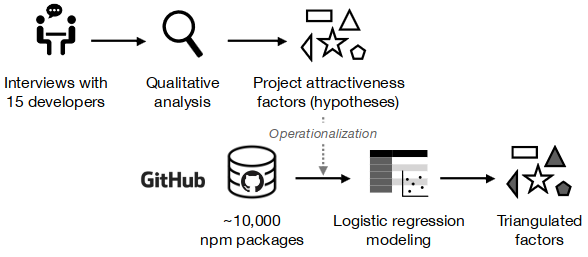
\includegraphics[width=\textwidth]{qiu_overview}
        \end{figure}
    \end{minipage}
    \begin{minipage}{.49\textwidth}
        \begin{figure}
            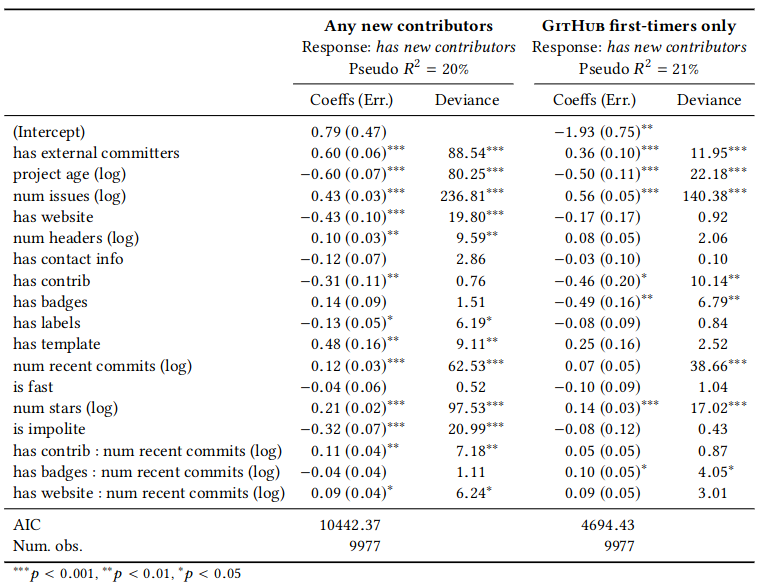
\includegraphics[width=\textwidth]{qiu_regressions}
        \end{figure}
    \end{minipage}

    % Je me suis beaucoup inspiré de cet article de Huilian Sophie Qiu et al.
    % qui identifie certains signaux que les aspirants contributeurs regardent
    % dans un projet pour choisir auquel contribuer, puis mesure la corrélation
    % qu'il y a entre ces signaux et la présence de tentative de contributions.

    % Ils trouvent en particulier qu'un grand nombre de \emph{commits} récents
    % est lié à une meilleur attractivité, contrairement à la présence
    % d'instructions de contribution. Leur étude mesure aussi de façon très
    % intéressante l'impact de la politesse des mainteneurs, ce que mon approche
    % ne me permettra pas de faire.

    % Notre but était de vérifier si certains de ces signaux marchent aussi pour
    % identifier les projets \emph{accessibles} (les contributeurs arrivent à
    % contribuer, leur code est intégré dans le projet) et non seulement
    % attractifs (les gens \emph{essayent} de contribuer).
    \note[item]{Inspiration principale : signaux d'attractivité}
    \note[item]{Par exemple HASCONTRIB négatif, recent commits positif}
    \note[item]{Est-ce que ces signaux prédisent aussi l'accessibilité ?}
\end{frame}

\section{Méthode}

\begin{frame}[fragile]{Pour dépasser les limites de GitHub}
    \mycite{mining-github-2014}, \mycite{penumbra-oss-2022} : limites du minage
    mono-plateforme.

    \smallskip

    \mycite{barriers-2018} : limites des études se concentrant sur quelques gros
    projets uniquement.

    \bigskip

    $\implies$ Besoin d'une stratégie de minage de données plus représentative
    et générique.

    \begin{figure}
        \includesvg[width=0.5\textwidth]{softwareheritage}
    \end{figure}

    % Autre objectif : dépasser les limites de l'analyse de données issues de
    % GitHub (beaucoup de projets "personnels", beaucoup de PR non marquées
    % comme \emph{merged} alors qu'elles l'ont été à la main, etc.).
    % Aussi beaucoup de projets très collaboratifs et actifs en dehors des
    % plateformes centralisées
    \note[item]{Github est la plateforme par défaut de ce genre d'études}
    \note[item]{Mais ses limites pour la recherche sont de plus en plus étudiées}
    \note[item]{Beaucoup de projets très collaboratifs existent en dehors des plateformes centralisées}
\end{frame}

\begin{frame}{Pertinence pour la recherche}
    \mycite{swh-2019}, \mycite{swh-seirl}.

    \begin{itemize}
        \item $+$\num{239000000} projets
        \item $+$\num{3000000000} \emph{commits} uniques
        \item Parcours régulièrement Bitbucket, GitHub, gitlab.com, CRAN, Maven,
            gnu.org, NPM, pypi, sourceforge, \ldots
        \item google code, autres GitLabs, autres origines à la demande
    \end{itemize}

    % Software Heritage maintient la plus grande archive logicielle publique au
    % monde avec l'objectif spécifique de la rendre exploitable à des fins de
    % recherche. L'archive contient des projets issus de nombreuses sources
    % différentes (GitHub restant la principale), y compris venant de logiciels
    % de versionnement différents, et tous représentés sous un seul grand graphe
    % de \emph{commits} dédupliqués.
    \note[item]{Plus grande archive logicielle entièrement publique du monde}
    \note[item]{Mise à disposition spécifiquement pour la recherche}
    \note[item]{Plus grande variété et exhaustivité}
\end{frame}

\begin{frame}{Un grand \emph{Merkle DAG}}
    \begin{minipage}{.46\textwidth}
        \begin{figure}
            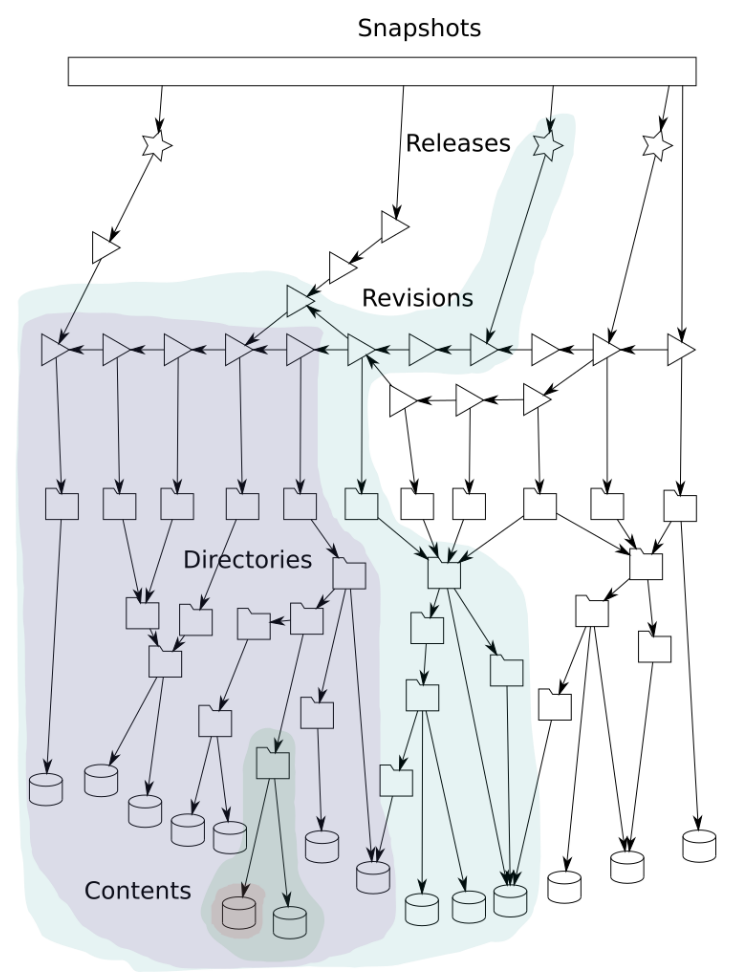
\includegraphics[width=\textwidth]{swh-graph}
        \end{figure}

        \mycite{swh-2019}
    \end{minipage}
    \begin{minipage}{.52\textwidth}
        Exclus de l'étude : \begin{itemize}
            \item les \emph{forks}
            \item les projets inactifs
            \item les projets non collaboratifs
        \end{itemize}

        \bigskip

        Données de recherche : \begin{itemize}
            \item nombre de nouveaux contributeurs (variable expliquée)
            \item nombre de contributeurs uniques récents
            \item nombre de \emph{commits} récents
            \item présence d'instructions de contribution
        \end{itemize}
    \end{minipage}
    
    % C'est un Merkle DAG, donc un graphe orienté sans cycle dont tous les nœuds
    % sont identifiés par un hash unique, ce qui permet de dédupliquer.

    % La vue ici est pour une "origine" (URL à partir de laquelle un archivage
    % peut être effectué). Les infos qui nous intéressent sont les snapshots
    % (date d'archivage), les révisions et, plus tard, les contenus des
    % fichiers.

    % Je commence donc par parcourir *tous* les nœuds du graphe, à chaque fois
    % que je trouve une origine je lance une découverte de composante connexe en
    % considérant aussi les arcs inverses des révisions (c'est à dire les
    % groupes de fork) ce qui me permet de sélectionner une origine
    % "représentante" des fork (celle la plus éloignée d'un \emph{commit}
    % initial) et d'éliminer toutes les autres de mon parcours.

    % Ensuite, pour chacun des projets retenus, je lance un parcours largeur à
    % partir de ce qui ressemble le plus à une branche principale afin de
    % récolter les données de recherche. Tout est prélevé uniquement au sein
    % d'une période de référence bien définie (et le caractère "récent" est une
    % autre période bien définie précédant la période de référence).
    \note[item]{Gigantesque graphe qui rassemble tous les historiques de tout le monde}
    \note[item]{Ici une vue depuis une seule "origine"}
    \note[item]{Premier parcours pour découvrir les origines (puis un de plus pour trouver les forks)}
    \note[item]{Ensuite récolte des données pour chaque projet retenu en partant d'une branche principale}
\end{frame}

\begin{frame}{Un \textbf{GRAND} \emph{Merkle DAG}}
    \centering

    Essentiellement trois parcours largeur
    \pause

    Entièrement en RAM (7 TiB), 48 cœurs
    \pause

    Structures et algorithmes optimisés, peu de synchronisation
    \pause
    \bigskip
    \bigskip

    {\huge Trois jours}\\{\footnotesize (et un jour de plus pour les READMEs)}

    % Software Heritage a été assez gentil pour faire tourner mon code sur leur
    % serveur capable de faire tenir tout le graphe en RAM, pendant deux
    % semaines où personne d'autre ne s'en servait j'ai pu utiliser les 48 cœurs
    % et paralléliser à fond.

    % Heureusement il y a des sous-graphes de taille raisonnable dont j'ai pu me
    % servir pour tester mon code de collecte chez moi)
    \note[item]{Le graphe est gros.}
    \note[item]{Il existe cependant des sous-graphes pour tester ses algos}
\end{frame}

\section{Résultats}

\begin{frame}{Instructions de contribution}
    \begin{figure}
        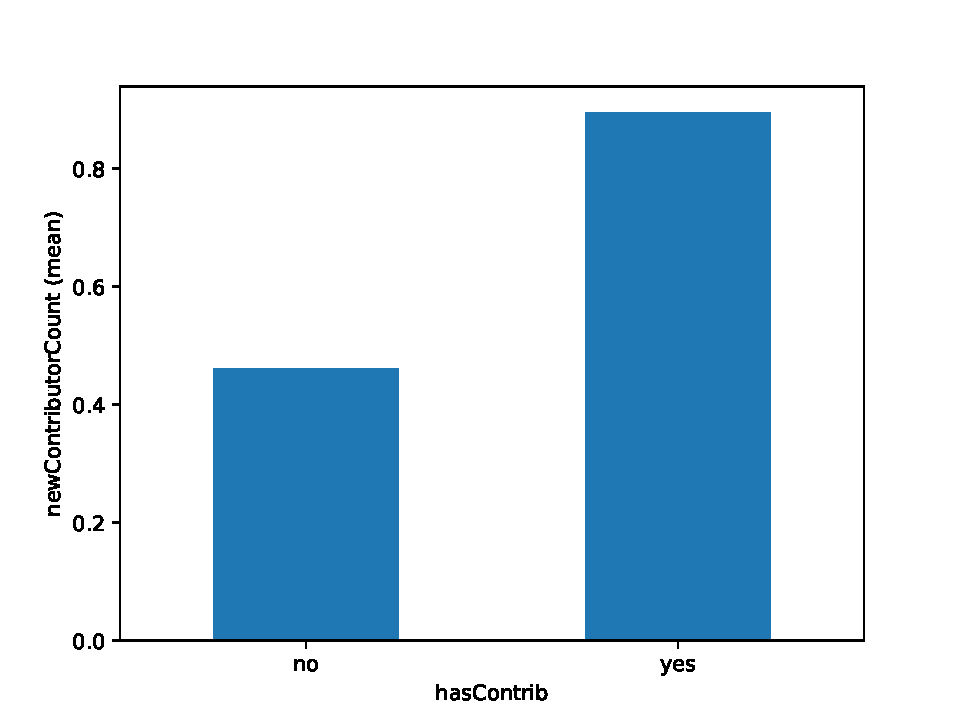
\includegraphics[width=.5\textwidth]{../experiment/data_analysis/hasContrib_meanNewContributorCount}
        \caption{%
            Moyenne du nombre de nouveaux contributeurs en fonction de la
            présence d'instructions de contribution
        }
    \end{figure}

    Test MWW : $\rho \approx 0.57$, $p \approx 0$

    \note[item]{%
        C'est très léger, mais d'après le test de Wilcoxon-Mann-Whitney il y a
        effectivement un lien entre la présence d'instructions de contribution
        d'un projet et son accessibilité pour les nouveaux contributeurs

        $p = 4.4591222 \times 10^{-135}$.
    }
\end{frame}

\begin{frame}{Nombre de contributeurs uniques récents}
    \begin{figure}
        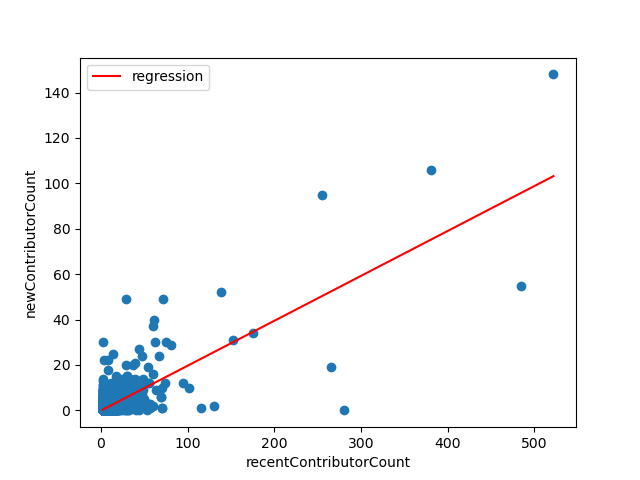
\includegraphics[width=.5\textwidth]{../experiment/data_analysis/recentContributorCountRegression_linearScale}
        \caption{%
            Nombre de nouveaux contributeurs en fonction du nombre de
            contributeurs uniques récents
        }
    \end{figure}

    Régression GLS : $R^2 \approx 0.45$

    \note[item]{%
        Là aussi c'est léger mais pareil, on voit un lien avec un coefficient de
        détermination de $45\%$. La difficulté c'est que la distribution des
        données n'est pas du tout normale, d'où l'utilisation d'un modèle
        utilisant la méthode des moindres carrés.
    }
\end{frame}

\begin{frame}{Nombre de \emph{commits} récents}
    \begin{figure}
        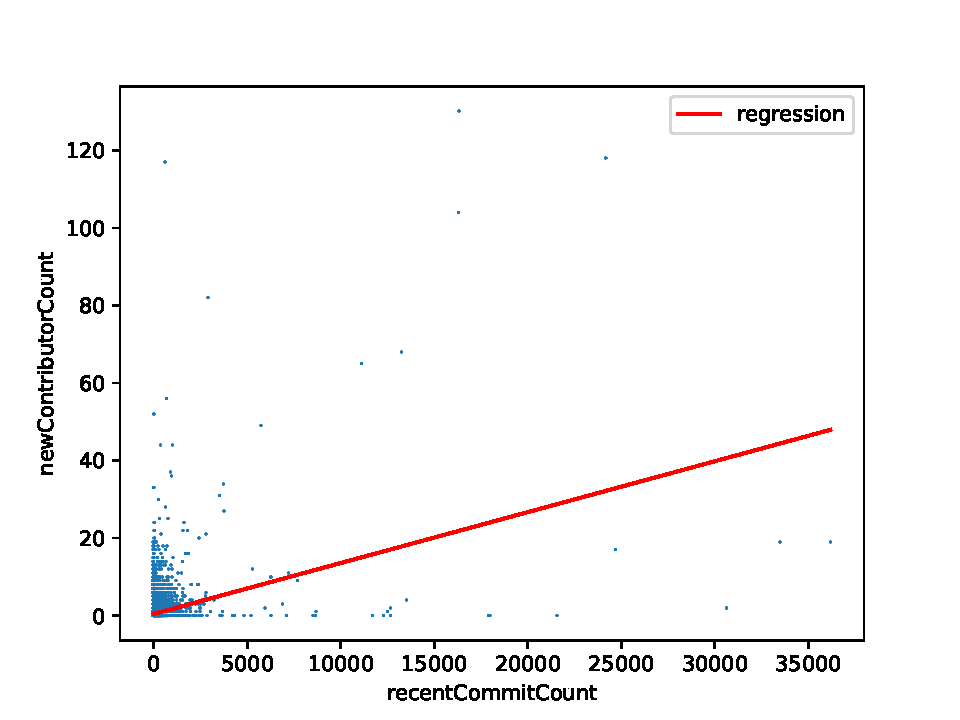
\includegraphics[width=.5\textwidth]{../experiment/data_analysis/recentCommitCountRegression_linearScale}
        \caption{%
            Nombre de nouveaux contributeurs en fonction du nombre de
            \emph{commits} récents
        }
    \end{figure}

    Régression GLS : $R^2 \approx 0.10$

    \note[item]{%
        Là c'est encore plus léger et le coefficient de détermination est à
        seulement $10\%$, c'est donc le seul lien que je ne retiens pas comme
        significatif.
    }
\end{frame}

\begin{frame}{Conclusion}
    Ceci n'était pas une publicité déguisée pour Software Heritage.
    \bigskip

    Limites : statistiques relativement faibles, absence d'information causale.

    Le logiciel libre est un gigantesque vivier de projets intéressants et
    "réels" où envoyer s'exercer des étudiants.
    \bigskip

    Des indicateurs semblent exister pour déterminer facilement lesquels sont
    accessibles aux nouveaux contributeurs, deux légers sont proposés dans cet
    article.

    \note[item]{%
        Ma présentation ressemble un petit peu à une pub pour Software Heritage,
        pourtant je vous assure que je ne suis pas sponsorisé. Mais je dois
        admettre que c'était très intéressant de travailler avec leur archive.

        En limite, les résultats sont quand même statistiquement assez faibles,
        et surtout on a aucune information causale.
    }
\end{frame}

\begin{frame}{Contact}
    \begin{itemize}
        \item Contact : \href{mailto:paul.hervot@epita.fr}{paul.hervot@epita.fr}
        \item Dépôt GitHub :
            \href{https://github.com/Dettorer/synva-dissertation}{Dettorer/synva-dissertation}
        \item \emph{Replication package} :
            \href{https://zenodo.org/record/7023495}{zenodo.org/record/7023495}
    \end{itemize}

    \note[item]{%
        La totalité du code utilisé dans l'article, ainsi que le LaTeX pour
        l'écrire lui-même, ainsi que les slides et le mémoire qui a servi de
        base, se trouvent dans ce repo github opensource, mais il y a aussi un
        replication package pour les gens souhaitant plus directement
        expérimenter avec le code de collecte et d'analyse des données. Je suis
        joignable à cette adresse mail et je serais, comme tout le monde
        j'imagine, bien évidemment très heureux de répondre à des questions si
        quelqu'un avait la curiosité d'aller regarder tout ça.
    }
\end{frame}

\section{Bibliographie}

\begin{frame}[allowframebreaks]{Bibliographie}
    \printbibliography{}
\end{frame}

\end{document}
